\documentclass[dvipdfmx]{jarticle}
\usepackage{graphicx}
\usepackage[top=30truemm,bottom=30truemm,left=25truemm,right=25truemm]{geometry}
\usepackage{listings,jvlisting}
\usepackage{url}

\lstset{
  basicstyle={\ttfamily},
  identifierstyle={\small},
  commentstyle={\smallitshape},
  keywordstyle={\small\bfseries},
  ndkeywordstyle={\small},
  stringstyle={\small\ttfamily},
  frame={tb},
  breaklines=true,
  columns=[l]{fullflexible},
  numbers=left,
  xrightmargin=0zw,
  xleftmargin=3zw,
  numberstyle={\scriptsize},
  stepnumber=1,
  numbersep=1zw,
  lineskip=-0.5ex
}

\makeatletter
\newcommand{\subsubsubsection}{\@startsection{paragraph}{4}{\z@}%
  {1.0\Cvs \@plus.5\Cdp \@minus.2\Cdp}%
  {.1\Cvs \@plus.3\Cdp}%
  {\reset@font\sffamily\normalsize}
}
\makeatother
\setcounter{secnumdepth}{4}

\begin{document}
\begin{titlepage}
    \begin{center}
        {\huge 情報科学演習D 課題4レポ―ト}
        \vspace{180pt}\\
        \begin{tabular}{rl}
            氏名 & 山久保孝亮\\
            所属 & 大阪大学基礎工学部情報科学科ソフトウェア科学コース\\
            メールアドレス & u327468b@ecs.osaka-u.ac.jp\\
            学籍番号 & 09B22084\\
            提出日 & \today\\
            担当教員 & 桝井晃基 松本真佑
        \end{tabular}
    \end{center}
\end{titlepage}
\section{システムの仕様}
課題4の外部仕様は以下のようになる.
\begin{itemize}
  \item 第一引数で指定されたtsファイルを読み込んで構文解析,意味解析,CASLのコード生成の順に処理を行う.コンパイル結果は第二引数で指定されたcasファイ
  ルに書き込む.
  \item コンパイルが成功した場合は文字列"OK"を返し,構文的,意味的誤りを検出した場合は各誤りの内容を返す.課題3のように複数の誤りがpasプログラムに含
  まれる場合は,一番最初に検出した誤りの内容を返す.また,誤りを最初に発見するとcasファイルを生成せず,入力ファイルが見つからない場合は文字列
  "File not found"を返す.
\end{itemize}
\section{課題達成の方針と設計}
今回の課題では,構文解析と意味解析を終了した際にグローバル変数として定義したリストresultDataにCASLのコードをadd()によって追加していく.このresultData
は"String型のリスト"のリストであり,例えば"CALL PROC0"というCASLコードの場合は["CALL","PROC0"]という二つの文字列の要素を持つリストを追加していた.
つまり,resultDataの各要素はCASLコード一行分を表す.
\\以下では,各処理におけるCASLコードの流れを記述する.
\subsection{変数の代入方法}
変数の代入は,純変数への代入と添字付き変数への代入に分類できる.
\begin{itemize}
  \item 純変数への代入の場合,
  \begin{enumerate}
    \item 指定する変数のアドレスとVARのアドレスの差を計算しGR2に格納する.
    \item スタックから右辺の値をPOPし,GR1に格納する.
    \item VARとGR2から実行アドレスを計算し,GR1に格納している値をストアする.
  \end{enumerate}
  という流れでCASLコードを追加する.1の差の計算方法は3.1の実装プログラムで記述する.また,VARは2.4で記述するようにメモリの先頭の番地である.
  \item 添字付き変数への代入の場合,
  \begin{enumerate}
    \item 右辺の構文定義"式"内で処理したCASLコードを追加する.
    \item 添え字を表す構文定義"式"内で処理したCASLコードを追加する.
    \item スタックから添え字の値をPOPし,GR2に格納する.
    \item 指定する配列のアドレスとVARのアドレスの差を計算し,GR2の値と加算し,GR2に格納する.これにより,指定したい配列の指定したいインデックス
    のアドレスを指定することができる.
    \item VARとGR2から実行アドレスを計算し,GR1に格納している値をストアする.
  \end{enumerate}
  という流れでCASLコードを追加する.
\end{itemize}
\subsection{式の処理方法}
式の処理によって生成されるCASLは,式に関係演算子が含まれる時と含まれない時に分類される.
\begin{itemize}
  \item 関係演算子が含まれない時,構文定義"単純式"内で処理されたCASLコードが追加される.このとき,単純式によって得られる値はスタックにPUSHされている.
  \item 関係演算子が含まれる時,一つ目の単純式と二つ目の単純式内でCASLコードが追加された後に,関係演算子の処理を実行するCASLコードを追加する.
  関係演算子を処理するCASLコードは以下のようになる.
  \begin{enumerate}
    \item スタックからGR1とGR2にそれぞれ一つ目の単純式と二つ目の単純式の結果をPOPする.
    \item GR1とGR2の値を比較する.このとき,CPLまたはCPAを使用する.
    \item それぞれの関係演算子によって,TRUE Xラベルにジャンプする.Xはラベルの番号を表す.
    \item 比較結果がfalseの時の処理を記述する.具体的には,GR1に\#0000を格納してBOTH Yラベルにジャンプする.Yもラベルの番号を表す
    \item 比較結果がtrueの時の処理を記述する.TRUEXラベルを付けた命令NOPの後に,GR1に\#FFFFを格納する.
    \item BOTHラベルを付けた命令NOPの後に,GR1の内容をPUSHする.
  \end{enumerate}
  という流れで処理が行われる.それぞれの処理を分岐させる方法については実装方法で記述する.また,TRUEXのXとBOTHYのYはラベルの管理方法で記述する.
\end{itemize}
  単純式によって生成されるCASLは加法演算子が含まれる時と含まれない時に分類できる.
  \begin{itemize}
    \item 加法演算子が含まれない時,
    \begin{enumerate}
      \item 構文定義"項"内で処理されたCASLコードが追加される.このとき,項によって得られる値はスタックにPUSHされている.
      \item 符号が「-」のとき,スタックから単純式の値をGR2にPOPし,GR1に0を格納する.そして,GR1からGR2の値を減算し,GR1に格納する.これにより,0-G
      R2という計算が実行され,負の数が実現できる.そして計算後の負の数をPUSHする.
    \end{enumerate}
    \item 加法演算子が含まれる時,加法演算子が含まれるときの処理の後に
    \begin{enumerate}
      \item 再び構文定義"項"内で処理されたCASLコードが追加される.
      \item スタックから加法演算子の第二項をPOPする.
      \item スタックから加法演算子の第一項をPOPする.
      \item 各加法演算子に対応する命令(ADDA,SUBA,OR)を実行し,結果をGR1に格納する.
      \item GR1の内容をスタックにPUSHする.
    \end{enumerate}
    という流れでCASLコードが追加される.この処理は構文定義より,0回以上繰り返される.
  \end{itemize}
  項内では,単純式内の"項"で追加されるCASLコードが"因子"で追加されるようになり,各加法演算子に対応する命令が各乗法演算子に対応する命令に変更される.
  変更後のCASLコードは以下の表1のようになる.
  \clearpage
  \begin{table}[h]
    \centering
    \begin{tabular}{|c||c|}
      \hline
      "*" & CALL MULTの後,GR2をPUSH\\\hline
      "/"または"div" & CALL DIVの後,GR2をPUSH\\\hline
      "mod" & CALL DIVの後,GR1をPUSH\\\hline
      "and" & ANDの後,GR1をPUSH\\\hline
    \end{tabular}
    \caption{単純式から変更された各乗法演算子に対応する処理}
  \end{table}
  因子では,「変数」,「定数」,「(式)」,「not 因子」の4種類に処理が分かれる.
  \begin{itemize}
    \item 変数の時,
    \begin{enumerate}
      \item VARからのアドレスの差を計算し,VARとアドレスの差を足し合わせた番地の値をGR1に格納する.
      \item GR1の値をスタックにPUSHする.
    \end{enumerate}
    という流れでCASLコードが追加される.
    \item 定数の時は,構文定義"定数"内でスタックに値がPUSHされる.PUSHされる内容は以下の表2のようになる.
    \begin{table}[h]
      \centering
      \begin{tabular}{|c||c|}
        \hline
        数値 & その数値の値\\\hline
        長さが1の文字列 & GR1に格納された1文字の文字列\\\hline
        true & \#FFFF\\\hline
        false & \#0000\\\hline
      \end{tabular}
      \caption{PUSHされる内容}
    \end{table}
    \item  (式)の時は,構文定義"式"内で処理されたCASLコードが追加される.
    \item not 因子のとき,
    \begin{enumerate}
      \item 因子内で処理されたCASLコードが追加される.
      \item スタックから因子の値をGR1にPOPする.
      \item \#FFFFとGR1の値をXORし,その結果をGR1に格納する.これにより,GR1の各ビットを反転させることができる.
      \item GR1の値をスタックにPUSHする.
    \end{enumerate}
    という流れでCASLコードが追加される.
  \end{itemize}
\subsection{手続きの呼び出し方法}
手続きの呼び出しは,
\begin{enumerate}
  \item 実パラメータをスタックにPUSHする.実パラメータが無ければ何もPUSHせずに次の処理を行う.
  \item 各手続きに対応するラベルをCALLする.CALLをするとスタックにプログラムレジスタの値を,つまり次に実行すべき命令語の先頭アドレスをPUSHする.
  \item GR1にスタックポインタを代入し,仮パラメータの個数を加算する.これにより,GR1がCALLを実行する前にPUSHした最初の実パラメータの値が格納されてい
  る番地を指すようになる.実パラメータがなければ0を加算し,以下の4からの処理は実行しない.
\end{enumerate}
という流れでCASLコードを追加する.
\subsection{ラベルの管理方法}
CASLコード内で使用されるラベルは以下の表のようになっている.
\begin{table}[h]
  \centering
  \begin{tabular}{|c||c|}
    \hline
    CASL & CASL文の記述の開始を表す\\\hline
    BEGIN & CASL文のプログラムの先頭を表す\\\hline
    LOOP & whileの条件式についての処理の先頭を表す\\\hline
    TRUE & while,ifの条件式がtrueの場合の処理を記述\\\hline
    BOTH & 
    \begin{tabular}{c}
      条件式の結果がtrueであればその後の構文定義"複合文",\\falseであればELSEにジャンプする処理の先頭を表す
    \end{tabular}\\\hline
    ENDLP & whileの終了を表す.その後はwhile文以降の処理が記述される\\\hline
    ELSE & 
    \begin{tabular}{c}
      if-elseでない場合はifの終了を表す.その後はif文以降の処理が記述される\\if-elseである場合はelse内の構文定義"複合文"の処理が記述される
    \end{tabular}\\\hline
    ENDIF & if-else文の終了を表す.その後はif-else文以降の処理を記述\\\hline
    PROC & 各副プログラムの先頭を表す\\\hline
    VAR & メモリの番地の先頭を表す\\\hline
    CHAR & 二文字以上の文字列の情報を格納\\\hline
  \end{tabular}\\
  \caption{ラベルの種類と内容}
\end{table}
\\LOOP,TRUE,BOTH,ENDLP,ELSE,ENDIF,PROC,CHARはその後,構文定義内で処理された順に0から1ずつ数値が増やされ分類される.即ち,if文が入れ子構造にな
っている場合は,ELSEやENDIFが登場するより前に複合文内でのifが処理されることになるため,CASLコード内で登場するラベルの順番は,TRUE0,BOTH0,TRUE1,
BOTH1,ELSE1,ELSE0のようになる.
\subsection{分岐の処理方法}
分岐の処理においては,構文定義"文"におけるif文,if-else文,while文内で処理が行われる.
\begin{itemize}
  \item while文のとき,
  \begin{enumerate}
    \item LOOP NOPを追加しwhile文の開始位置を決める
    \item 2.2の構文定義"式"における,関係演算子が含まれる場合の処理によりCASLコードが追加される.
    \item スタックから条件式の結果(trueまたはfalse)をGR1にPOPする.
    \item GR1と\#0000(false)が一致しているかをCPLにより確認し,一致してればゼロフラグが立つ.
    \item JZEにより,ゼロフラグが立っていればENDLPにジャンプする.
    \item 構文定義"複合文"内で処理されたCASLコードが追加される.
    \item LOOPにジャンプする.即ち,1からこの処理を再び行う.
    \item ENDLP NOPを追加しwhile文の処理が終了する
  \end{enumerate}
  という流れでCASLコードが追加される.
  \item if文の場合,
  \begin{enumerate}
    \item 2.2の構文定義"式"における,関係演算子が含まれる場合の処理によりCASLコードが追加される.
    \item スタックから条件式の結果(trueまたはfalse)をGR1にPOPする.
    \item GR1と\#0000(false)が一致しているかをCPAにより確認し,一致してればゼロフラグが立つ.
    \item JZEにより,ゼロフラグが立っていればELSEにジャンプする.
    \item 構文定義"複合文"内で処理されたCASLコードが追加される.
    \item ELSE NOPを追加しif文の処理が終了する.
  \end{enumerate}
  という流れでCASLコードが追加される.
  \item if-else文の場合,
  \begin{enumerate}
    \item if文の1から5と同様の処理が行われる.
    \item ENDIFにジャンプする.
    \item ELSE NOPを追加し,その後elseの際の構文定義"複合文"内で処理されたCASLコードが追加される.
    \item ENDIF NOPを追加しif-else文の処理が終了する.
  \end{enumerate}
  という流れでCASLコードが追加される.
\end{itemize}
\subsection{レジスタやメモリの利用方法}
各レジスタの利用方法は以下の表のようになる.
\begin{table}[h]
  \centering
  \begin{tabular}{|c||c|}
    \hline
    GR1 & 様々な用途に用いられるバッファ\\\hline
    GR2 & 様々な用途に用いられるバッファ\\\hline
    GR3 & スタックにPUSHされている実パラメータのアドレスの内容を格納\\\hline
    GR6 & 0番地のアドレスを格納\\\hline
    GR7 & LIBBUFのアドレスを格納\\\hline
    GR8 & スタックポインタ\\\hline
  \end{tabular}
  \caption{各レジスタとその利用方法}
\end{table}
\\また,メモリの仕様及び利用方法は以下のようになる.
\begin{itemize}
  \item メモリの仕様はVARがメモリの先頭を表し,まずグローバル変数の領域がDSにより確保される.以降,各副プログラムごとに仮パラメータ,ローカル変数の
  領域が格納される.また,変数の領域の直後のアドレスから,二文字以上の文字列をDCにより格納される.各文字列はCHARとその後に0から始まる数値を結合したものを
  ラベルとして持つ.最後に,LIBBUFというラベルとともにDSにより256個の領域が確保される.
  \item メモリの利用方法は2.1のように参照する変数とメモリの先頭であるVARのアドレスの差を計算してその差をVARと加算することで実行アドレスを計算する.
  具体的な処理方法は3.2で記述する.
\end{itemize}
\subsection{スコープの管理方法}
各仮パラメータのスコープの管理は,2.3の副プログラムが呼び出された後に処理される.具体的には,
\begin{enumerate}
  \item 「PUSHされた実パラメータのアドレス」の中身即ち実パラメータの値をGR2に格納し,DSで確保した領域にその値を格納する.
  \item GR1の値を1減らす.これは,4で指定した実パラメータの次のアドレスを表す.3の時点で最後の実パラメータでなければGR1は次の実パラータのアドレスを
  ,3の時点で最後の実パラメータの値であればGR1は2のプログラムレジスタの値を指す.
  \item 1,2を繰り返す.繰り返しが終了するとGR1にプログラムレジスタの値を格納する.この後は複合文のCASLを記述する.
  \item スタックポインタに実パラメータのサイズを加算した値をGR8に格納する.これにより,1でPUSHする前のスタックのアドレスをスタックポインタが指すようになる.最後に,GR1をスタックポインタに格納し,RETする.
  これにより,プログラムレジスタの値に格納されているアドレスの処理が実行されるようになる.
\end{enumerate}
という流れでCASLコードが追加される.
\subsection{過去の課題プログラムの再利用}
手続き内で定義された変数に関する情報(識別子名,型,サイズ)はリスト型のグローバル変数として定義している.具体的には,グローバル変数について格納する
global\_variable\_tableとローカル変数について格納するlocal\_variable\_tableを定義している.ローカル変数表は直前に定義した副プログラムのローカル変数
の情報のみを格納するため,複数の副プログラムを定義した場合,以前の変数の情報が失われてしまっていた.そこで,新たにローカル変数表を格納するリストlocal
\_variable\_table\_listを作成することで複数のローカル変数表の情報を記憶できるようになった.
\section{実装プログラム}
ここでは,2で記述したCASLコードを記述するためのプログラム内での処理について記述する.
\subsection{各ラベルの数字の管理方法}
2.4で記述したLOOP,TRUE,BOTH,ENDLP,ELSE,ENDIF,PROCはそれぞれint型のグローバル変数としてX\_countとして定義した.Xは前述の各ラベルが入る.また,
各構文定義を処理するメソッド内ではローカル変数this\_X\_countにX\_countを代入し,処理が終わると使用したグローバル変数を1インクリメントする.これにより
,入れ子構造の際のラベルの管理は以下の図のようになる.
\begin{figure}[h]
  \centering
  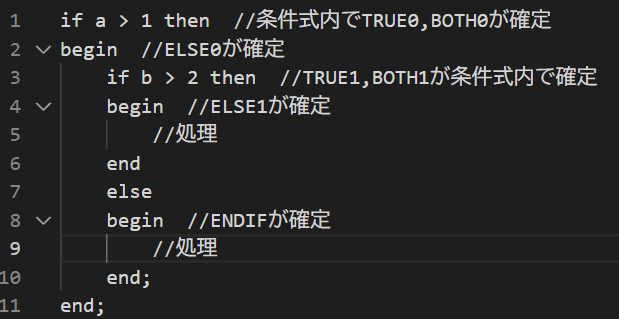
\includegraphics[width = 8cm]{ireko.png}
  \caption{入れ子構造におけるラベルの管理}
\end{figure}
\\上図のラベルが確定しているのは,this\_X\_countに代入されたことを表す.11行目の「end;」でELSE0に関する処理を記述するが,ローカル変数として定義
しているため,内側のif文の影響を受けてELSE2となるのではなく,ELSE0として記述することができる.
\subsection{変数の参照の際のVARとのアドレスの差の計算方法}
2.6より,メモリにはグローバル変数,仮パラメータ,ローカル変数の順で領域が確保されている.また,仮パラメータとローカル変数は一つの副プログラムに対して
1セットで確保されるため,二つ以上の副プログラムが定義されている場合は,グローバル変数,仮パラメータ,ローカル変数,仮パラメータ,ローカル変数...と
いう順番で領域が確保される.また,参照する変数は,「グローバル変数」,「ローカル変数または仮パラメータ」,「副プログラム内で参照されるグローバル変数」,
「添字付き変数」の4つに分類できる.それぞれの処理は,以下のように行う.
\begin{itemize}
  \item グローバル変数の場合は,グローバル変数表から順に参照していき,対象の識別子と変数表内の識別子が一致するまで各変数のサイズを加えることで計算
  する.具体的には,以下のようなプログラムで実行される.
  \begin{lstlisting}
for(variable list : global_variable_table) {
  if(list.getName().equals(name)) {
    break;
  }
sum = sum + list.getSize();
}
  \end{lstlisting}
  これにより,対象の識別子と変数表中の識別子が一致するまでのサイズを計算できる.
  \item ローカル変数または仮パラメータの場合は,各ローカル変数表において,対象の変数までのサイズとグローバル変数表の全ての変数のサイズを足し合わせる.
  このとき,各副プログラムのローカル変数を格納した表は定義された副プログラムの順に参照される.つまり,副プログラムf1とf2が存在し,f2中の変数を参照した
  い場合はまずf1のローカル変数表のサイズを全て足してからf2の変数表を参照し,対象の変数までのサイズを計算する.その後,グローバル変数表の全変数のサイズ
  を足し合わせる.具体的には,以下のようなプログラムで記述される.
  \begin{lstlisting}
if(local_variable_table_list.size() != 0) {
  for(ArrayList<variable> table : local_variable_table_list) {
    for(variable list : table) {
      if(list.getName().equals(name) && (count == proc_count)) {
          local = true;
          for(variable list1 : global_variable_table) {
              sum = sum + list1.getSize();
            }
          break;
        }
        sum = sum + list.getSize();
    }
      count++;
    }
}
  \end{lstlisting}
  localは,falseに初期化されているboolean型の変数であり,countは0に初期化されているint型の変数である.countは現在何番目に定義したローカル変数表を参照
  しているのかを表しており,4行目の条件式より,proc\_countと一致した時のみグローバル変数の全サイズを足し合わせる.localは前述の処理が起こったとき,即ち
  参照する変数がローカル変数であったときにtrueとなる.
  \item 副プログラム内でグローバル変数を参照する場合は,まず上記のローカル変数の参照と同様の処理を行う.そして,以下の処理を追加で行う.
  \begin{lstlisting}
if(local == false) {
  sum = 0;
  //
グローバル変数と同じ処理を行う}
  \end{lstlisting}
  ローカル変数表に対する処理を事前に行い,sumの値が変更されているのでまずsumを0に初期化している.そして,グローバル変数のときと同様の処理を行っている.
  \item 添字付き変数の時は,上記と同様の方法で計算してから1を引く.
\end{itemize}
のように分けることができる.
\subsection{副プログラムのCASLコードの処理順序}
副プログラムの処理は,構文解析や意味解析を行う際は,
\[構文定義"副プログラム"内の処理→構文定義"プログラム"内の複合文の処理\]
という順で処理が実行される.しかし,CASLコードの場合は,
\[構文定義"プログラム"内の処理→構文定義"副プログラム"内の複合文の処理\]
という順でコードが追加される.\\
この違いを解決するために,グローバル変数として"String型のリスト"のリストproc\_casl\_listを定義した.これには,構文定義"副プログラム宣言群"の一回の繰り
返しの中で追加されたCASLコードが格納される.また,このときresultDataのCASLコードは削除されている.\\
CASLコードの追加方法は,各副プログラム宣言の前と後にresultDataのサイズをsize()により取得し,subList()を使って抜き出した.また,resultDataにproc\_casl
\_listの内容を追加するのは構文定義"プログラム"内の複合文の後である.これにより,上記のCASLコードの順番で追加することができる.
\subsection{添字付き変数への代入の際の処理順序}
添字付き変数への代入は,構文解析や意味解析を行う際は,
\[変数名(配列名)→式(添字)→右辺の式\]
という順で処理が実行される.しかし,CASLコードの場合は,
\[右辺の式→式(添字)→変数名(配列名のアドレス計算)\]
の順に処理が実行される.\\
この処理の違いを解決するために,グローバル変数として"String型のリスト"のリストleft\_index\_casl\_listを定義した.これには,
構文解析における"式"内で追加されるCASLコードを格納しておく.そして,CASLコードの"右辺の式"の処理が行われてからresultDataに追加する.\\
具体的な追加の方法としては,3.3で記述したproc\_casl\_listへの追加方法と基本的には同じである.ただ,添え字付き変数への代入における添え字の"式"のみに
対して処理を行いたいため,添え字付き変数への代入であることを示すフラグをグローバル変数として定義した.
そして2.1のように添え字付き変数への代入の処理を追加していく.
\\
ところで,添字を表す構文定義"式"内で"(式)"が含まれる時,即ち"式"の中に入れ子構造で再び"式"がある場合,上述の通り添字を表す"式"で追加されるCASLコードは
一旦別のリストに格納される.このとき,どの"式"の処理が終了した段階でCASLコードを別のリストに格納するかを判定する必要がある.そこで,first\_index\_flag
というグローバル変数と,first\_flagというローカル変数を定義する.そして,添字を表す構文定義"式"の処理メソッドを呼び出す直前で前者をtrueに設定する.
メソッド内では,後者に前者の値を格納し,前者をfalseとする.これにより,このメソッド内ではfirst\_flagはtrueとなり,今後入れ子構造になっている"式"が
呼び出されたときはグローバル変数がfalseとなっているためfirst\_flagはfalseとなる.これにより,first\_flagを使うことでこの問題を解決できる.
\subsection{スコープ管理の処理}
スコープ管理は,2.7より,実パラメータのサイズと,参照する実パラメータのアドレスを計算する必要がある.
\begin{itemize}
  \item 実パラメータのサイズは,3.2と同様にしてローカル変数表のサイズを足し合わせparameter\_sizeに格納して実現した.このとき,VARからのアドレスの差
  ではなくサイズの合計のみ知ることができればよいので直前のローカル変数表のみを参照すればよい.
  \item 3.2の仮パラメータの処理を行い,sumに格納した.
\end{itemize}
また,2.7の1と2は仮パラメータごとに繰り返して処理されるため,上記で計算したsumの値を繰り返しごとに1ずつ増やしていくことで実現した.
\section{考察}
今回の課題を通して,特定の場合の処理を行う場合はフラグを使用することで処理を分岐させた.フラグを用いて処理を分岐させること欠点は,「フラグの数が増える
と,プログラムの処理の分岐が増加し可読性が下がってしまうこと」が挙げられる.この欠点を解決するための工夫として,以下のようなものが考えられる.
\begin{itemize}
  \item フラグの名称だけで何を目的としたフラグなのかが分かるようにする.例えば,flag1のような名称にしてしまうと,何のためのフラグなのかが分からなく
  なってしまうが,「isGrobalVariable」等の名称にすれば,trueとfalseがこの変数名への返答となり,名称を見るだけでtrueの場合はグローバル変数について
  記述するということが分かるようになり,可読性が向上する.
  \item 各フラグを構造体として定義する.これによりフラグの数が増加した際も管理しやすくなる.また,新しいフラグを追加する際の修正箇所が限定され,可読性
  が向上する.
\end{itemize}

\section{感想}
この講義全体を通して,計画的に課題を進めることができたと感じた.今後の学習及び研究においても長期的に計画を立てて学習を進めていきたいと思う.
\begin{thebibliography}{99}
    \bibitem{1} 言語処理工学A 講義スライド
    \bibitem{2} 情報科学演習D 指導書
\end{thebibliography}
\end{document}